\chapter{Ischemic Heart Disease}
\label{ihd-background}

Ischemic heart disease is a term covering a variety of conditions, 
all caused by myocardial ischemia---%
an imbalance between the coronary blood supply and the 
oxygen requirements of the myocardium.
In the overwhelming majority of cases, 
this imbalance can be attributed to obstructive atherosclerotic disease 
that limits coronary blood flow
~\autocite{kumarRobbins2017}.
In these cases, ischemic heart disease is therefore synonymous 
with coronary artery disease.

The central etiological entity in ischemic heart disease
is therefore the atherosclerotic plaque, 
which is part of the process known as atherosclerosis. 
An atherosclerotic plaque consists of blood cells, lipids, calcium 
and connective tissue that are gradually deposited in the arterial wall 
over a number of years.
~\autocite{kumarRobbins2017}
The plaque can grow large enough to severely narrow the arterial lumen,
or it can become unstable and as a consequence rupture or erode,
leading to thrombosis.
Both of these scenarios can severely affect 
the perfusion of tissues and organs, 
and when coronary arteries are affected,
it can lead to ischemic heart disease.

\begin{figurefw}
    \centering
    \vspace{-5em}
	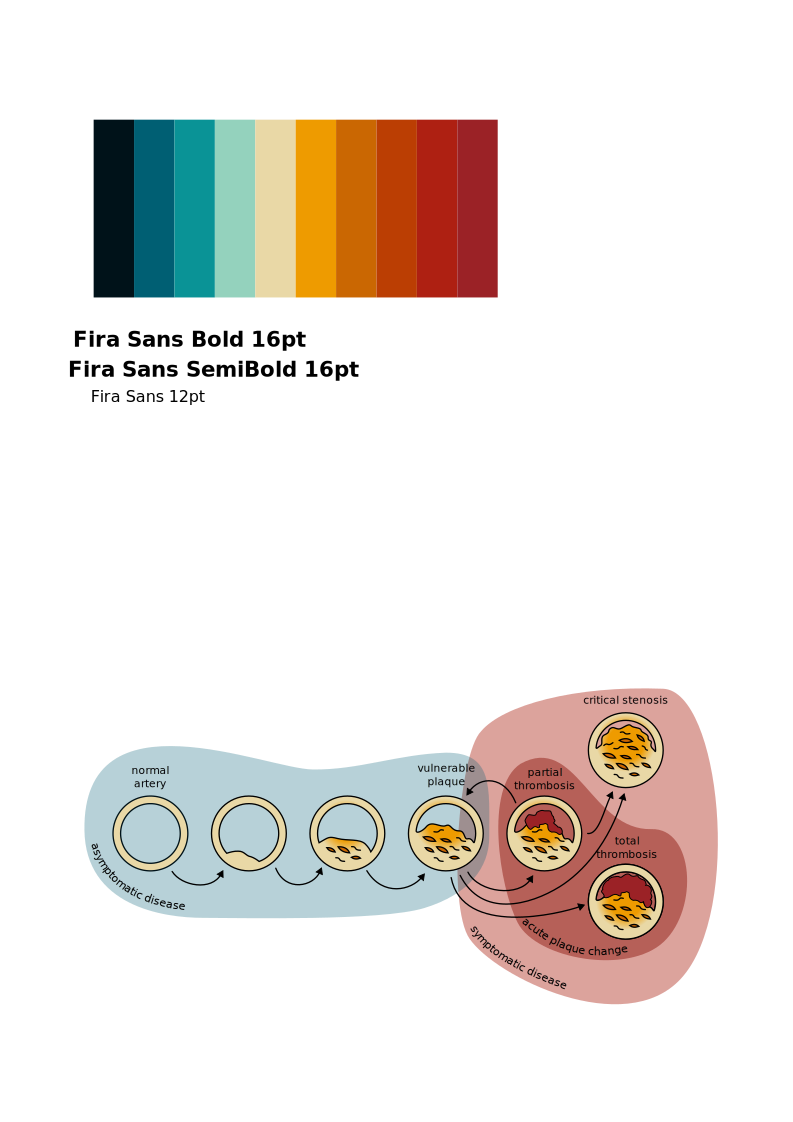
\includegraphics[width=\linewidth]{graphics/atherosclerosis}
    \caption[The process of atherosclerosis]{%
        \textit{Critical stenosis} represents the tipping point at which
        the gradual occlusion of the arteries leads to onset of symptoms.
        While the patient may be asymptomatic at rest, 
        increased physical activity results in cardiac ischemia and  
        intense chest pain.
        \textit{Acute plaque change} is the sudden rupture or erosion of 
        the atherosclerotic plaque which triggers thrombosis.
        The resulting thrombus can partially or completely fill the vascular
        lumen.
        Disruption of endothelial integrity.
    }
    \label{OneOfMyMissingFigures}
\end{figurefw}

\vskip 10em
%------------------------------------------------------------------------------

\section{Manifestation}

The underlying pathological process is inherently chronic,
but ischemic heart disease can abruptly transition to an acute condition.
Often, the disease is initially identified when this acute transition 
has already happened.




The clinical presentation of ischemic heart disease include
both chronic and acute manifestations of myocardial ischemia. 

\begin{table}
    \begin{tabular}{ll}\toprule
        Syndrome              & Manifestation \\\midrule
        Angina Pectoris       & Description \\
        Myocardial Infarction & Description \\\bottomrule
    \end{tabular}
\end{table}




\section{Prevalence}

\todo[inline]{Danish statistics on IHD incidence and prevalence.}



Angina pectoris, myocardial infarction, chronic IHD, and sudden cardiac death.

Chronic ischemic heart disease is a syndrome characterised by
gradual heart failure following ischemic myocardial injury.

Inflammation.
Endothelial cells and circulating leukocytes.
T-cell and macrophage recruitment and activation.
Smooth muscle cell accumulation. 



Typical or stable angina is episodic but consistent chest pains
linked to physical activity.
Unstable angina, is as its name indicate more variable, and 
is usually characterized by an increase in frequency and intensity
of chest pain.

Myocardial infarction is caused by acute thrombosis following 
sudden ruption or erosion of an atherosclerotic plaque.



The central entity in the etiology of ichemic heart disease 
is the atherosclerotic plaque. 

Fate of the atherosclerotic plaque



Atherosclerotic plaques can, 
as they increase in size, occlude the vascular lumen 
and mechanically affect the circulation.


In coronary atherosclerosis, 
The abnormal, often turbulent, blood flow in the vicinity of atherosclerotic
plaques can, in combination with the loss of endothelial integrity, lead to
formation of arterial thromboses.
~\autocite{kumarRobbins2017}

Such thromboses can embolise, but may also increase in size and gradually 
occlude the vascular supply of the heart.
The consequences of the occlusion can,
depending on the local vascular anatomy and extent of the occlusion,
range from relatively benign to extensive tissue necrosis
and even death~\autocite{kumarRobbins2017}.

\section{Consequences and Complications}
\section{Co-morbidity}
\section{Diagnosis}
\section{Complications}
\section{Treatment}

If the occlusion of one coronary artery happens slowly, 
it can allow time for the development of collateral blood supplies,
which might prevent myocardial infarction
~\autocite{kumarRobbins2017}.
